\documentclass{article}
\usepackage{graphicx}
\usepackage{amsmath}
\usepackage{amsfonts}
\usepackage{amssymb}
\usepackage{amsthm}
\usepackage{xcolor}
\usepackage{geometry}[margin={1cm,1cm}]

\newtheorem{thm}{Theorem}
\newtheorem{lem}[thm]{Lemma}
\newtheorem{cor}[thm]{Corollary}
\newtheorem{defn}[thm]{Definition}

\author{Ben Shirley}

\begin{document}
\section*{Question 1}

\begin{enumerate}

\item \begin{enumerate}
    \item $\{a, b, d\}$
    \item $\{e, f, g, h\}$
    \item $\{a, b, e, g, h\}$
\end{enumerate}

\item This is a rank 4 matroid, and circuits are minimal non-independent sets. Any 5-element subset of a 6+-element set is a depenendent set, 
    and so no 6+-element set can be a circuit. M has no copunctual points, so no two elements are depenendent. Hence $M$ has no 2-element circuits.
\item 
\begin{enumerate}
    \item $\{d, b, i, e\}$.
    \item $\emptyset$
    \item $\{a, b, c, d, e, f, g, h, i\}$
    \item $\{d, g, i, f, e\}$ - any 4 element subset is coplanar, but d, g, i is independent.
\end{enumerate}
\end{enumerate}
\section*{Question 2}
$(i)\implies (ii)$: If $\{e\}\in\mathcal{C}(M)$, then $\{e\}\not\in\mathcal{I}(M)$. If $e\in B\in\mathcal{B}(M)$ for some basis, 
then $\{e\}\subseteq B\in \mathcal{I}(M)$, and so $\{e\}\in \mathcal{I}(M)$, a contradiction.
Hence $e$ is not in any basis.

$(ii)\implies (iii)$: Suppose that $e$ is not in any basis of $M$. Then $\mathcal{I}(M)=\{Y\subseteq E: Y\subseteq B\in\mathcal{B}\}$.
Since $x\not\in B$ for any basis, and all independent sets are subsets of a basis, $x\not\in Y$ for any $Y\in\mathcal{I}(M)$.

$(iii)\implies (i)$: Suppose $e$ is in no independent set. Then $\{e\}\not\in \mathcal{I}(M)$, so is depenendent. But then $\emptyset\in\mathcal{I}(M)$,
so $\{e\}$ is a minimal depenendent set, and so is a circuit (hence $e$ is a loop).

\section*{Question 3}
By thm 1.7 it suffices to show that $\mathcal{I}$ satisfies I1-3.
\begin{enumerate}
    \item[I1] $\emptyset\in I_1 ,I_2$. So $\emptyset=\emptyset\cup\emptyset\in\mathcal{I}$.
    \item[I2] Let $Y=Y_1\cup Y_2\in\mathcal{I}$, and suppose $X\subseteq Y$. Now $X=X\backslash Y_2\cup X\backslash Y_1$,
    since $E_1, E_2$ are disjoint.
        But $X\backslash Y_2\subseteq Y\backslash Y_2\subseteq Y_1\in I_1$, and $X\backslash Y_1\subseteq Y\backslash Y_1\subseteq Y_2\in I_2$.
        So  $X\backslash Y_2\in I_1$ and $X\backslash Y_1\in I_2$, by applying I2 to each matroid.
        Thus $X=X\backslash Y_2\cup X\backslash Y_1\in\mathcal{I}$.
    \item[I3] Let $X=X_1\cup X_2, Y=Y_1\cup Y_2\subseteq \mathcal{I}$, with $|X|<|Y|$.
         Assume w.l.o.g. that  $|Y_1|>|X_1|$ (We have at least one of this, or $|Y_2|>|X_2|$, so just swap the two if not).
            Then  by the independence augmentation property of $I_1$, 
         $\exists y\in Y_1\backslash X_1$, such that $X_1\cup y\in I_1$. 
         Then we have found some $y\in Y_1\backslash X_1\subseteq Y\backslash X$,
         such that $X\cup y=(X_1\cup y)\cup X_2\in\mathcal{I}$.
         (Note again that $E_1$ and $E_2$ are disjoint).
\end{enumerate}

\section*{Question 4}
    This is false. Consider $E=\{1, 2, 3, 4, 5, 6\}$, and $C'=\{\{1, 2, 3, 4\}, \{1, 2, 5, 6\}\}$, defining $B_{4, C'}$ as our bases (as per the next question).
    So our bases for this matroid are the $4$-element sets not in $C'$, and in particular, we see that $\{3, 4, 5, 6\}$ is one of them.
    However, $\{1, 2, 3, 4\}$ and $\{1, 2, 5, 6\}$ are depenendent sets, and it is easy to see that any subset of either is contained in a basis set.
    So they are circuits.

    Then we have $\{1, 2, 3, 4\}\cap \{1, 2, 5, 6\}\ne\emptyset$, and yet $\{1, 2, 3, 4\}\Delta\{1, 2, 5, 6\}=\{3, 4\}\cup\{5, 6\}=\{3, 4, 5, 6\}$,
    which is a member of $B_{4, C'}$ and so not a circuit!

\section*{Question 5}
Let $E$ be a finite set, and let $r$ be an integer with $0 < r < |E|$. Let $C'$ be a collection of r-
element subsets of $E$ such that if $C_1$ and $C_2$ are distinct members of $C$, then $|C_1 \cap C_2| <
r - 1$. Let $B_{r,C'}$ be the family of $r$-element subsets of $E$ that are not in $C'$; that is,
$B_{r, C'} = {B \subseteq E : |B| = r and B \not\in C'}.$
\begin{enumerate}
    \item $(E, B_{r, C'})$ is a matroid: First B1 is trivial! Suppose $\mathcal{C}'$ contained every $r$-element subset of $E$. Then taking any two $r$-element 
        subsets that differ by only one element, say $C_1, C_2$, we have that $|C_1\cap C_2|=r-1\not<r-1$. Hence at least one of the two subsets
        cannot be in $C'$. So some $r$-element subset is not in $\mathcal{C}'$,
        and is thus in $B_{r, C'}$ (and therefore it is non-empty).

        For B2, take $B_1, B_2\in B_{r, C'}$. Then take $x\in B_1\backslash B_2$. Now say that for each $y\in B_2\backslash B_1$, we have that $(B_1\backslash x)\cup y\not\in B_{r, C'}$,
        that is, $(B_1\backslash x)\cup y\in C'$. For any distinct $y_1, y_2\in B_2\backslash B_1$, notice that we have $((B_1\backslash x)\cup y_1)\cap ((B_1\backslash x)\cup y_2)= B_1\backslash x$.
        This has cardinality $r-1$, which contradicts the property of $C'$. So, if there are multiple elements in $B_2\backslash B_1$, at least one of the 
        sets obtained by basis exchange is not in $C'$, and is hence in $B_{r, C'}$. It remains to consider the case where $|B_2\backslash B_1|=1$.
        In this case, we have that $B_2 = (B_2\cap B_1)\cup (B_2\backslash B_1)$. Clearly these sets are disjoint, and thus we have $r=|B_2|=|B_2\cap B_1|+ |B_2\backslash B_1|$.
        But then it follows from $|B_2\backslash B_1|=1$ that $|B_2\cap B_1|=r-1$.

        Thus, we see that $|B_1\backslash B_2|=1$, and therefore $B_1\cap B_2=B_1\backslash \{x\}= B_2\backslash \{y\}$.
        So finally, we have that $(B_1\backslash x)\cup y= (B_2\backslash y)\cup y= B_2\not\in C'$. Hence the basis exchange property holds, and so $(E, B_{r, C'})$ is a matroid!


    \item Let $J(n, r)$ be the simple graph with r-element subsets of $1, ..., n$ as its verticies and 2 verticies adjacent iff the cardinality of their intersection is $r-1$.
        \begin{figure}[!htb]
           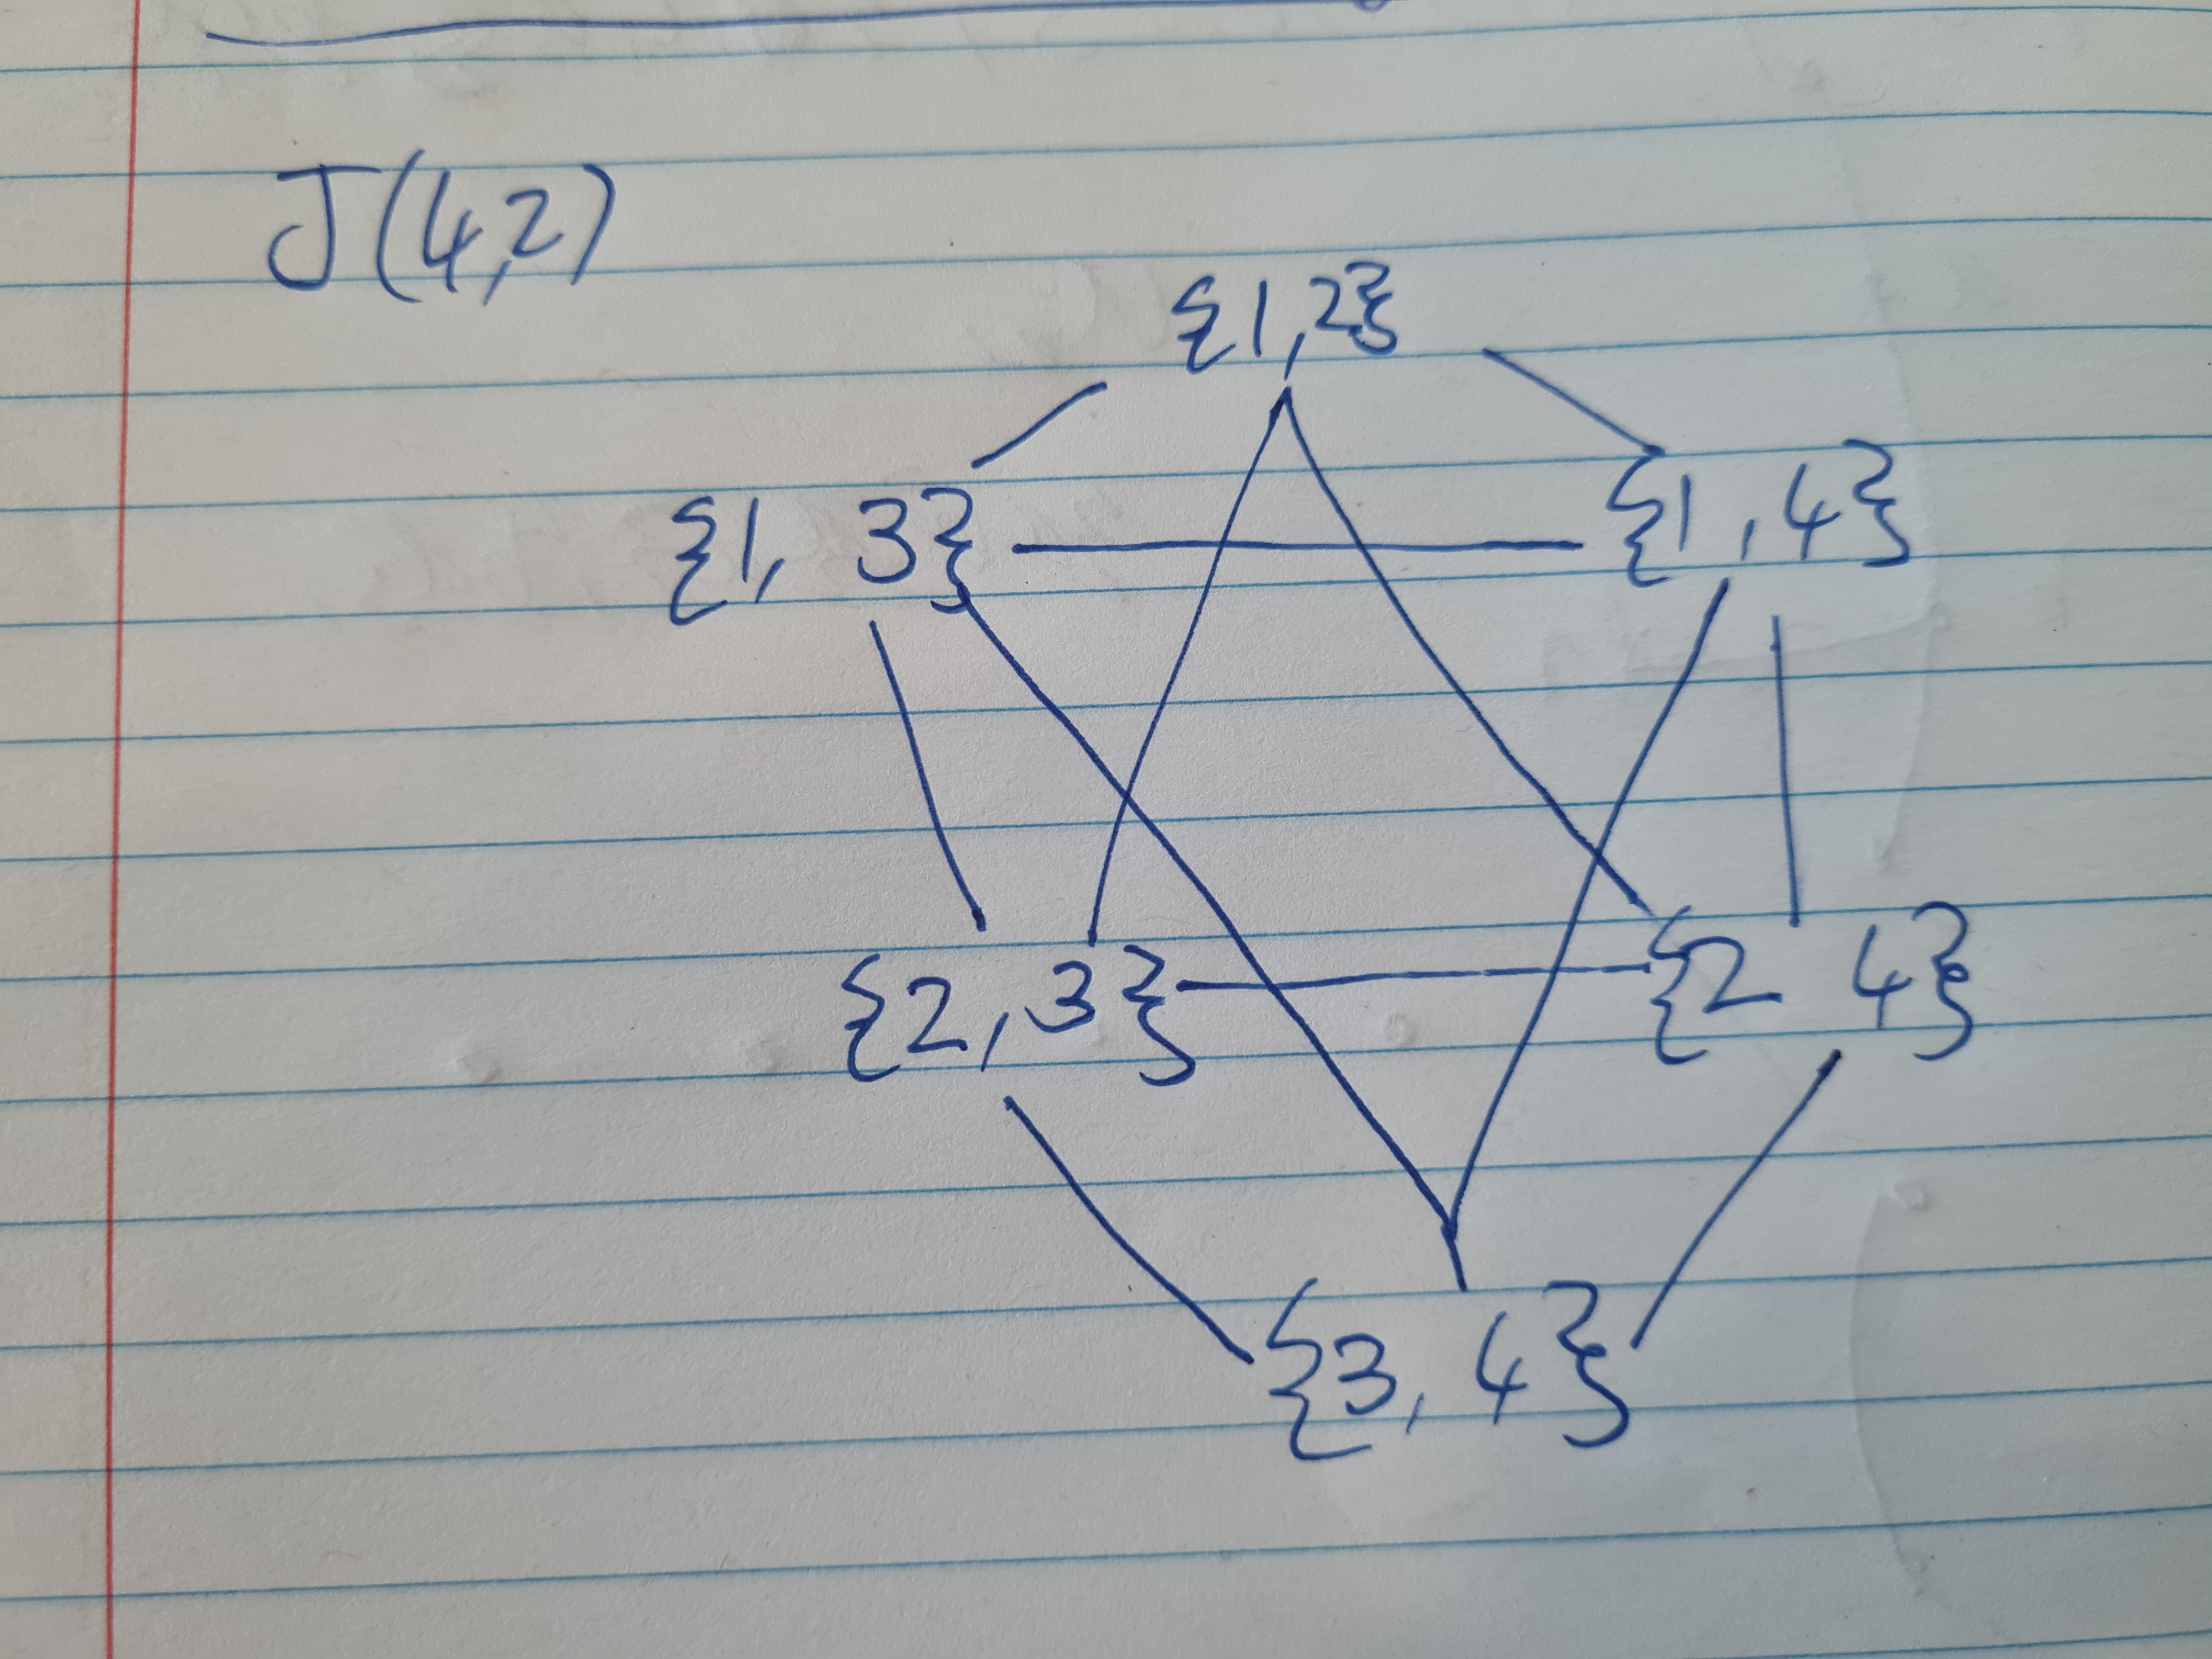
\includegraphics[width=0.5\textwidth]{j42.jpg}
        \end{figure}
        Stable sets of this graph look like disjoint partitions of $\{1, 2, 3, 4\}$. Since we connect two sets (in this case)
         iff they share 1 element in common, in order for two verticies to not be connected, they should not share any elements at all!
         So our stable sets are partitions of $\{1, 2, 3, 4\}$ into 2 two-element subsets.
    \item Clearly we have $U_{2, 4}$, since this is the uniform matroid of rank 2. It remains to list matriods of the form $(\{1, 2, 3, 4\}, B_{r, C'})$.
        In this case, we need $r=2$, and $C'$ is a collection of 2 element subsets such that for any distinct $C_1, C_2\in C'$, we have $|C_1\cap C_2|< 2-1$
        (or in other words, equal to 0). So, we could have $C'=\{\{1, 2\}\}$, or $\{\{1, 2\}, \{3, 4\}\}$. Clearly any other choices of $C'$ are isomorphic, 
        we just relabel the elements in the sets. This relabeling will then produce the corresponding matriod. So, these are all the rank 2, sparse paving matroids 
        on 4 elements.
    \begin{figure}
        \includegraphics[width=0.5\textwidth]{20250723_102053.jpg}
    \end{figure}
    \begin{figure}
        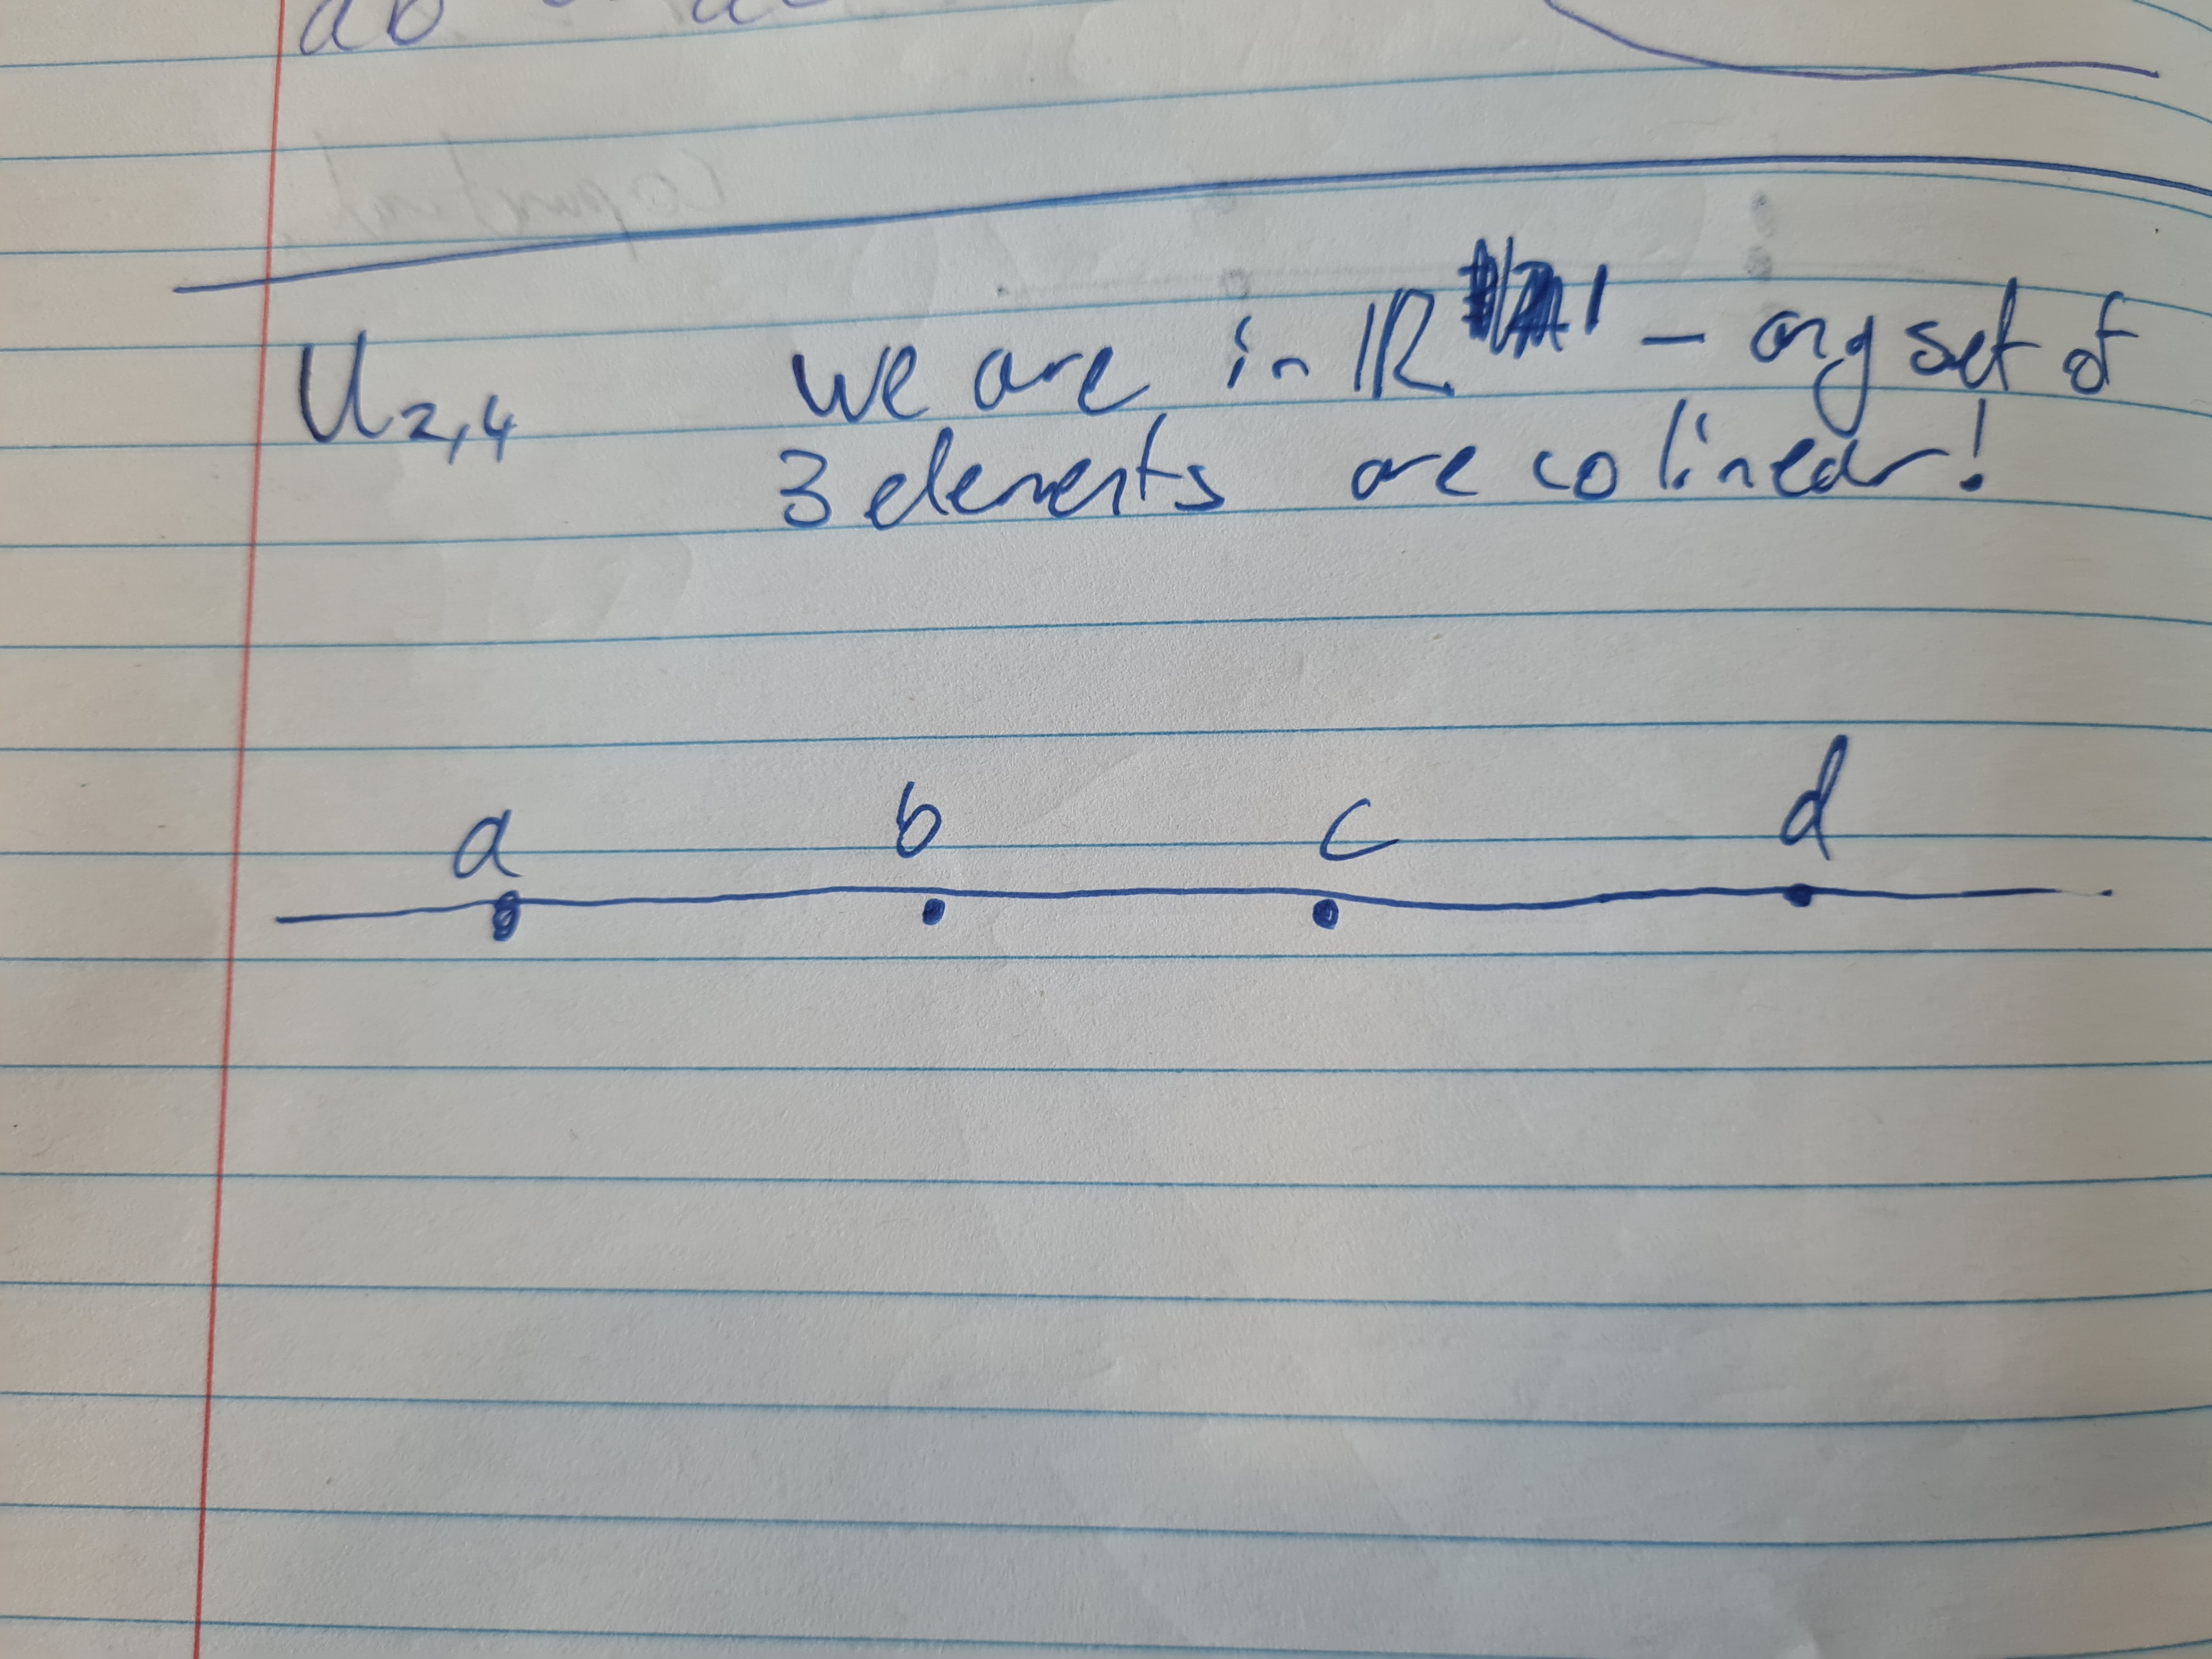
\includegraphics[width=0.5\textwidth]{20250723_102058.jpg}
    \end{figure}
\end{enumerate}

\end{document}